\documentclass{article}
\usepackage[utf8]{inputenc}
\usepackage[T1]{fontenc}
\usepackage{geometry}
\usepackage{tikz}
\usepackage{pgfplots}
\usepackage{amsmath}
\usepackage{xcolor}

\usetikzlibrary{shapes.geometric, arrows, positioning, patterns}
\pgfplotsset{compat=1.18}

\geometry{margin=1in}

\title{TikZ and Graphics Test}
\author{Docker Test Suite}
\date{\today}

\begin{document}

\maketitle

\section{Basic TikZ Drawings}

\subsection{Simple Shapes}
\begin{center}
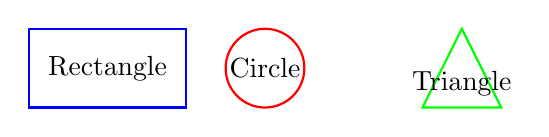
\begin{tikzpicture}
    % Rectangle
    \draw[thick, blue] (0,0) rectangle (2,1);
    \node at (1,0.5) {Rectangle};

    % Circle
    \draw[thick, red] (3,0.5) circle (0.5);
    \node at (3,0.5) {Circle};

    % Triangle
    \draw[thick, green] (5,0) -- (6,0) -- (5.5,1) -- cycle;
    \node at (5.5,0.3) {Triangle};
\end{tikzpicture}
\end{center}

\subsection{Flowchart}
\begin{center}
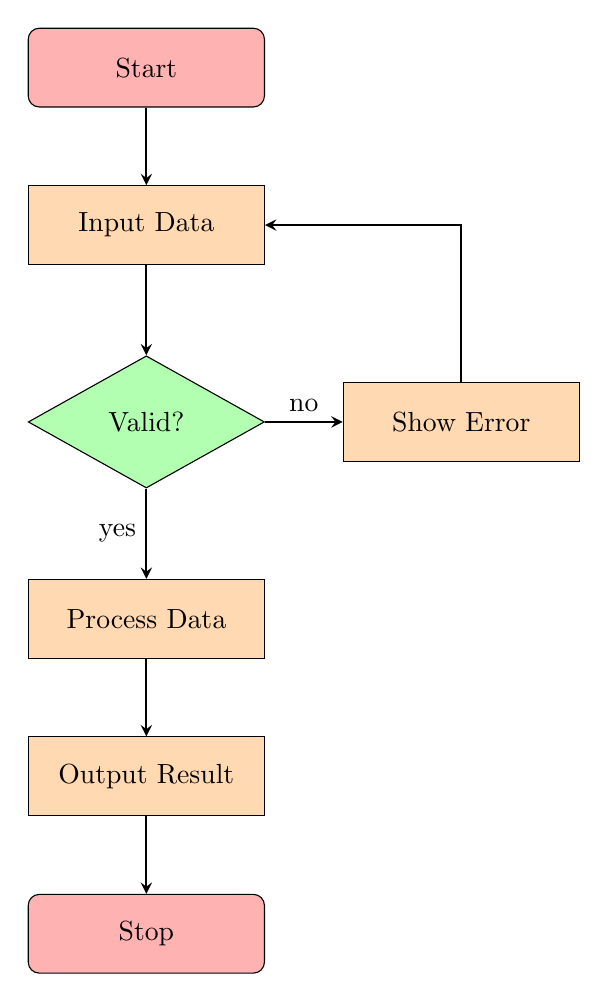
\begin{tikzpicture}[
    node distance=2cm,
    startstop/.style={rectangle, rounded corners, minimum width=3cm, minimum height=1cm, text centered, draw=black, fill=red!30},
    process/.style={rectangle, minimum width=3cm, minimum height=1cm, text centered, draw=black, fill=orange!30},
    decision/.style={diamond, minimum width=3cm, minimum height=1cm, text centered, draw=black, fill=green!30},
    arrow/.style={thick,->,>=stealth}
]

\node (start) [startstop] {Start};
\node (input) [process, below of=start] {Input Data};
\node (decide) [decision, below of=input, yshift=-0.5cm] {Valid?};
\node (process1) [process, below of=decide, yshift=-0.5cm] {Process Data};
\node (output) [process, below of=process1] {Output Result};
\node (stop) [startstop, below of=output] {Stop};
\node (error) [process, right of=decide, xshift=2cm] {Show Error};

\draw [arrow] (start) -- (input);
\draw [arrow] (input) -- (decide);
\draw [arrow] (decide) -- node[anchor=east] {yes} (process1);
\draw [arrow] (decide) -- node[anchor=south] {no} (error);
\draw [arrow] (process1) -- (output);
\draw [arrow] (output) -- (stop);
\draw [arrow] (error) |- (input);

\end{tikzpicture}
\end{center}

\section{Mathematical Plots with PGFPlots}

\subsection{Function Plot}
\begin{center}
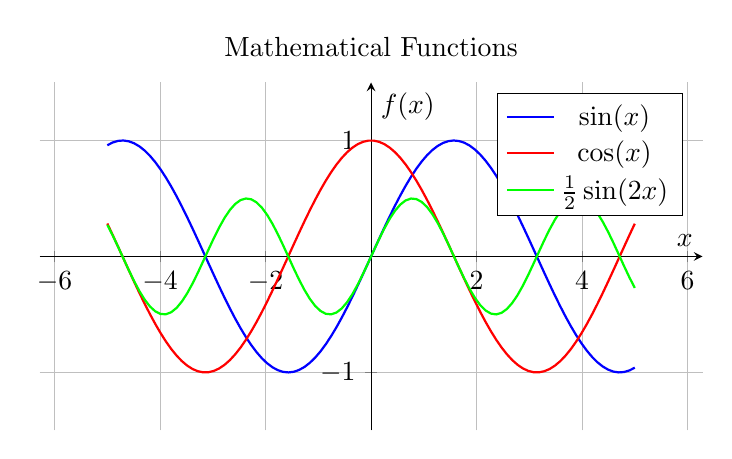
\begin{tikzpicture}
\begin{axis}[
    title={Mathematical Functions},
    xlabel={$x$},
    ylabel={$f(x)$},
    xmin=-2*pi, xmax=2*pi,
    ymin=-1.5, ymax=1.5,
    axis lines=middle,
    grid=major,
    width=10cm,
    height=6cm,
    legend pos=north east
]

\addplot[blue, thick, samples=100] {sin(deg(x))};
\addlegendentry{$\sin(x)$}

\addplot[red, thick, samples=100] {cos(deg(x))};
\addlegendentry{$\cos(x)$}

\addplot[green, thick, samples=100] {0.5*sin(deg(2*x))};
\addlegendentry{$\frac{1}{2}\sin(2x)$}

\end{axis}
\end{tikzpicture}
\end{center}

\subsection{Data Plot}
\begin{center}
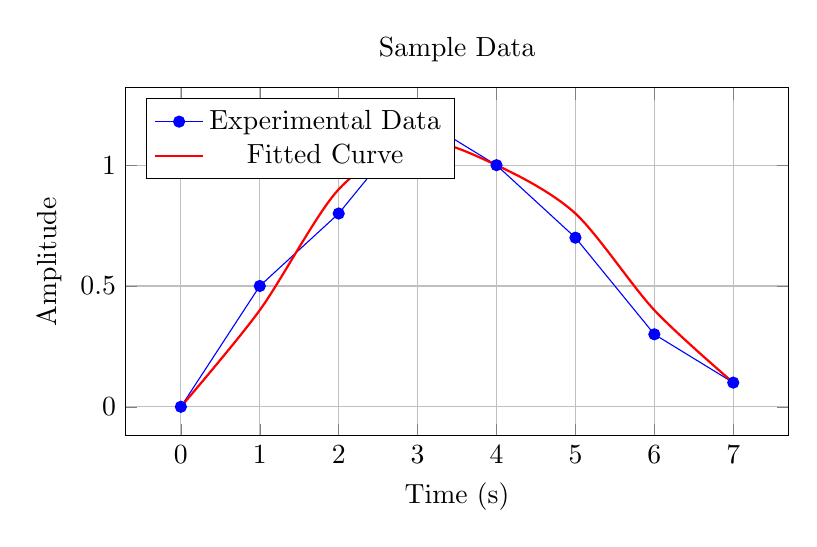
\begin{tikzpicture}
\begin{axis}[
    title={Sample Data},
    xlabel={Time (s)},
    ylabel={Amplitude},
    grid=major,
    width=10cm,
    height=6cm,
    legend pos=north west
]

\addplot[blue, mark=*, mark size=2pt] coordinates {
    (0,0) (1,0.5) (2,0.8) (3,1.2) (4,1.0) (5,0.7) (6,0.3) (7,0.1)
};
\addlegendentry{Experimental Data}

\addplot[red, thick, smooth] coordinates {
    (0,0) (1,0.4) (2,0.9) (3,1.1) (4,1.0) (5,0.8) (6,0.4) (7,0.1)
};
\addlegendentry{Fitted Curve}

\end{axis}
\end{tikzpicture}
\end{center}

\section{Complex Diagrams}

\subsection{Network Diagram}
\begin{center}
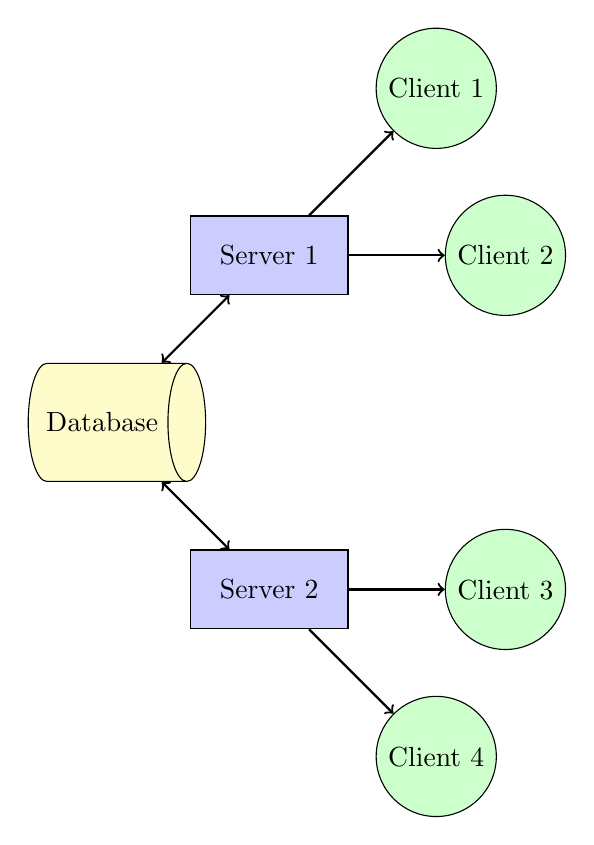
\begin{tikzpicture}[
    node distance=3cm,
    server/.style={rectangle, draw, fill=blue!20, minimum width=2cm, minimum height=1cm},
    client/.style={circle, draw, fill=green!20, minimum size=1cm},
    database/.style={cylinder, draw, fill=yellow!20, minimum width=1.5cm, minimum height=1cm}
]

\node (db) [database] {Database};
\node (server1) [server, above right of=db] {Server 1};
\node (server2) [server, below right of=db] {Server 2};
\node (client1) [client, above right of=server1] {Client 1};
\node (client2) [client, right of=server1] {Client 2};
\node (client3) [client, right of=server2] {Client 3};
\node (client4) [client, below right of=server2] {Client 4};

\draw[thick, <->] (db) -- (server1);
\draw[thick, <->] (db) -- (server2);
\draw[thick, ->] (server1) -- (client1);
\draw[thick, ->] (server1) -- (client2);
\draw[thick, ->] (server2) -- (client3);
\draw[thick, ->] (server2) -- (client4);

\end{tikzpicture}
\end{center}

\section{Geometric Constructions}

\begin{center}
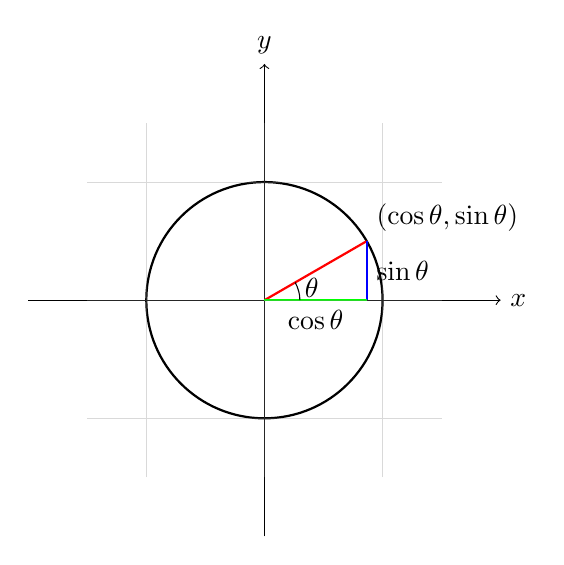
\begin{tikzpicture}[scale=1.5]
    % Draw coordinate system
    \draw[->] (-2,0) -- (2,0) node[right] {$x$};
    \draw[->] (0,-2) -- (0,2) node[above] {$y$};

    % Draw unit circle
    \draw[thick] (0,0) circle (1);

    % Draw angle
    \draw[thick, red] (0,0) -- (0.866,0.5);
    \draw[thick, blue] (0.866,0) -- (0.866,0.5);
    \draw[thick, green] (0,0) -- (0.866,0);

    % Mark angle
    \draw (0.3,0) arc (0:30:0.3);
    \node at (0.4,0.1) {$\theta$};

    % Labels
    \node[above right] at (0.866,0.5) {$(\cos\theta, \sin\theta)$};
    \node[below] at (0.433,0) {$\cos\theta$};
    \node[right] at (0.866,0.25) {$\sin\theta$};

    % Grid
    \draw[help lines, opacity=0.3] (-1.5,-1.5) grid (1.5,1.5);
\end{tikzpicture}
\end{center}

\section{Conclusion}
This document successfully demonstrates advanced graphics capabilities:
\begin{itemize}
    \item Basic TikZ shapes and drawings
    \item Complex flowcharts and diagrams
    \item Mathematical function plotting with PGFPlots
    \item Data visualization
    \item Network and system diagrams
    \item Geometric constructions
\end{itemize}

All TikZ and PGFPlots functionality is working correctly in the full variant.

\end{document}